\documentclass{nime-alternate} % Uncomment when publishing final version
% Uncomment when publishing final version
% \documentclass{nime-alternate}
% \usepackage{anonymize}
%\usepackage[blind]{anonymize}
\usepackage[utf8]{inputenc}
\usepackage{hyperref}

\usepackage{color}
\usepackage{fancyvrb}
\newcommand{\VerbBar}{|}
\newcommand{\VERB}{\Verb[commandchars=\\\{\}]}
\DefineVerbatimEnvironment{Highlighting}{Verbatim}{commandchars=\\\{\}}
\usepackage{framed}
\definecolor{shadecolor}{RGB}{240,240,240}
\newenvironment{Shaded}{\begin{snugshade}}{\end{snugshade}}
\newcommand{\AlertTok}[1]{\textcolor[rgb]{0.94,0.16,0.16}{#1}}
\newcommand{\AnnotationTok}[1]{\textcolor[rgb]{0.56,0.35,0.01}{\textbf{\textit{#1}}}}
\newcommand{\AttributeTok}[1]{\textcolor[rgb]{0.77,0.63,0.00}{#1}}
\newcommand{\BaseNTok}[1]{\textcolor[rgb]{0.00,0.00,0.81}{#1}}
\newcommand{\BuiltInTok}[1]{#1}
\newcommand{\CharTok}[1]{\textcolor[rgb]{0.31,0.60,0.02}{#1}}
\newcommand{\CommentTok}[1]{\textcolor[rgb]{0.56,0.35,0.01}{\textit{#1}}}
\newcommand{\CommentVarTok}[1]{\textcolor[rgb]{0.56,0.35,0.01}{\textbf{\textit{#1}}}}
\newcommand{\ConstantTok}[1]{\textcolor[rgb]{0.00,0.00,0.00}{#1}}
\newcommand{\ControlFlowTok}[1]{\textcolor[rgb]{0.13,0.29,0.53}{\textbf{#1}}}
\newcommand{\DataTypeTok}[1]{\textcolor[rgb]{0.13,0.29,0.53}{#1}}
\newcommand{\DecValTok}[1]{\textcolor[rgb]{0.00,0.00,0.81}{#1}}
\newcommand{\DocumentationTok}[1]{\textcolor[rgb]{0.56,0.35,0.01}{\textbf{\textit{#1}}}}
\newcommand{\ErrorTok}[1]{\textcolor[rgb]{0.64,0.00,0.00}{\textbf{#1}}}
\newcommand{\ExtensionTok}[1]{#1}
\newcommand{\FloatTok}[1]{\textcolor[rgb]{0.00,0.00,0.81}{#1}}
\newcommand{\FunctionTok}[1]{\textcolor[rgb]{0.00,0.00,0.00}{#1}}
\newcommand{\ImportTok}[1]{#1}
\newcommand{\InformationTok}[1]{\textcolor[rgb]{0.56,0.35,0.01}{\textbf{\textit{#1}}}}
\newcommand{\KeywordTok}[1]{\textcolor[rgb]{0.13,0.29,0.53}{\textbf{#1}}}
\newcommand{\NormalTok}[1]{#1}
\newcommand{\OperatorTok}[1]{\textcolor[rgb]{0.81,0.36,0.00}{\textbf{#1}}}
\newcommand{\OtherTok}[1]{\textcolor[rgb]{0.56,0.35,0.01}{#1}}
\newcommand{\PreprocessorTok}[1]{\textcolor[rgb]{0.56,0.35,0.01}{\textit{#1}}}
\newcommand{\RegionMarkerTok}[1]{#1}
\newcommand{\SpecialCharTok}[1]{\textcolor[rgb]{0.00,0.00,0.00}{#1}}
\newcommand{\SpecialStringTok}[1]{\textcolor[rgb]{0.31,0.60,0.02}{#1}}
\newcommand{\StringTok}[1]{\textcolor[rgb]{0.31,0.60,0.02}{#1}}
\newcommand{\VariableTok}[1]{\textcolor[rgb]{0.00,0.00,0.00}{#1}}
\newcommand{\VerbatimStringTok}[1]{\textcolor[rgb]{0.31,0.60,0.02}{#1}}
\newcommand{\WarningTok}[1]{\textcolor[rgb]{0.56,0.35,0.01}{\textbf{\textit{#1}}}}

\newlength{\cslhangindent}
\setlength{\cslhangindent}{1.5em}
\newenvironment{cslreferences}%
  {\setlength{\parindent}{0pt}%
  \everypar{\setlength{\hangindent}{\cslhangindent}}\ignorespaces}%
  {\par}

\begin{document}

\conferenceinfo{NIME'20,}{July 21-25, 2020, Royal Birmingham Conservatoire, ~~~~~~~~~~~~ Birmingham City University, Birmingham, United Kingdom.}
\title{Algorithmic Pattern}

\numberofauthors{1}
%
\author{
\alignauthor
Alex McLean\\
       \affaddr{Research Institute for the History of Science and Technology}\\
       \affaddr{Deutsches Museum, Munich}\\
       \email{alex@slab.org}
}

\date{31st January 2020}

\maketitle
\begin{abstract}
This paper brings together two main perspectives on algorithmic
pattern. First, the writing of musical patterns in live coding
performance, and second, the weaving of patterns in textiles. In both
cases, algorithmic pattern is an interface between the human and the
outcome, where small changes have far-reaching impact on the results.

By bringing contemporary live coding and ancient textile approaches
together, we reach a common view of pattern as algorithmic movement
(e.g. looping, shifting, reflecting, interfering) in the making of
things. This works beyond the usual definition of pattern used in
musical interfaces, of mere repeating sequences. We conclude by
considering the place of algorithmic pattern in a wider activity of
making.

\end{abstract}

\keywords{Pattern, TidalCycles, Algorithmic Music, Textiles, Live Coding, Algorave}

%% \begin{CCSXML}
%% <ccs2012>
%%    <concept>
%%        <concept_id>10010405.10010469.10010475</concept_id>
%%        <concept_desc>Applied computing~Sound and music computing</concept_desc>
%%        <concept_significance>500</concept_significance>
%%        </concept>
%%    <concept>
%%        <concept_id>10010405.10010469.10010471</concept_id>
%%        <concept_desc>Applied computing~Performing arts</concept_desc>
%%        <concept_significance>500</concept_significance>
%%        </concept>
%%    <concept>
%%        <concept_id>10010405.10010469.10010474</concept_id>
%%        <concept_desc>Applied computing~Media arts</concept_desc>
%%        <concept_significance>500</concept_significance>
%%        </concept>
%%    <concept>
%%        <concept_id>10011007.10011006.10011008.10011009.10011012</concept_id>
%%        <concept_desc>Software and its engineering~Functional languages</concept_desc>
%%        <concept_significance>300</concept_significance>
%%        </concept>
%%  </ccs2012>
%% \end{CCSXML}

\ccsdesc[500]{Applied computing~Sound and music computing}
\ccsdesc[500]{Applied computing~Performing arts}
\ccsdesc[500]{Applied computing~Media arts}
\ccsdesc[300]{Software and its engineering~Functional languages}

% this line creates the CCS Concepts section.
\printccsdesc

\hypertarget{defining-algorithmic-pattern}{%
\section{Defining algorithmic
pattern}\label{defining-algorithmic-pattern}}

This paper explores the world of algorithmic pattern, and the ways in
which it offers an interface to the computer musician. To introduce this
topic, let's first look at the words \emph{pattern} and \emph{algorithm}
separately, before putting them together.

\sloppypar

Patterns are present everywhere, certainly in textiles, choreography,
mathematics, design and music. However, at first glance, the use of the
word \emph{pattern} in music seems comparatively impoverished, at least
in the West. At the time of writing, the English language Wikipedia page
on pattern has no mention of music, and when musicians talk about
pattern, they usually mean any sequence that repeats. The word can even
take on a pejorative sense in music, for example in a conference paper
on transdisciplinary collaboration Hugill recounts how (and I
paraphrase) mathematicians devote their careers to searching for
patterns, whereas many composers will be seriously offended if you
accuse them of making patterns.\footnote{Hugill's paper is unpublished
  but a video of its presentation is available at
  \href{https://medias.ircam.fr/x6e2d95}{medias.ircam.fr/x6e2d95} with
  follow-on blog
  \href{http://www.andrewhugill.com/blog/?p=3159}{andrewhugill.com/blog/?p=3159}
  (both accessed 30 Jan 2020).}

This paper compares patterns in music with those in textiles. The
textile arts and crafts are alive with compositional patterning
techniques, not only repetitions but reflections and symmetries, and
generative structural compositions. Once you scratch the surface of
music, it is of course also fully alive with patterns. As just one
example, consider \emph{canon} structures, where one voice imitates
another, played over the top with a delay - an example of rotational or
glide symmetry. So it seems that the difference here is the way words
are used; in music, a canon \emph{contains} patterns, whereas in
textiles, such a structure would \emph{itself} be referred to as the
pattern.

So what \emph{is} a Pattern? Grünbaum and Shephard (1986) define
patterns as ``designs repeating some motif in a more or less systematic
manner.'' They write in the context of geometric tilings, but the same
definition largely holds in music fields; a sequence becomes a pattern,
once it is repeated. However, in music we too often focus on the
\emph{repetition}, and not the \emph{systematic manner} in which it is
repeated. For a pattern to be interesting, we need to do more than
repeat it; the repetition only provides the metrical ground on which the
pattern acts. Looking around the room you are in now, you will likely
see patterns of repetition, but also of reflection, rotation,
interference/moire, and glitches or deviations from those patterns. The
textiles around (or on) you may well have a visual pattern arising not
from the colour of threads alone, but from computational interference
between colour and structure.

Accordingly, in the present paper, \emph{pattern} is taken to refer to a
whole family of techniques for working with regularities in the world.
Such patterns allow us to perceive repetition, reflection and
interference in a material. In other words, the way we perceive pattern
is inextricably linked with the structured movements of its making. And,
once we are dealing with `structured movements of making', we are in the
world of algorithms.

An \emph{algorithm} is a step-by-step set of instructions. Sometimes it
is assumed that by a step-by-step set, we mean a sequence of
instructions, but this is not the case; indeed the notion of an
algorithm has been formalised as lambda calculus, which may involve
recursive steps \emph{into} a function declaration, rather than stepping
\emph{down} a stateful sequence of statements. This clarification
becomes important later in this paper, when we address TidalCycles, a
live coding environment embedded in the Haskell language, which is
itself based on lambda calculus.

There is some sense that as used in this paper the words
\emph{algorithm} and \emph{pattern} are synonyms; they both refer to
structured ways of making. Therefore the phrase ``algorithmic pattern''
seems to be a tautology. The phrase is nonetheless useful for on one
hand clarifying that we address algorithms not just as software
engineering tools, but as formalised ways of making that can to a large
extent be perceived in end-results. It also clarifies that we are
interested in patterns that are not just simple sequences, but
structural qualities. This builds a perspective on pattern as a
generative and perceptual connection between creation and reception. In
short, I define algorithmic pattern as the perception of systematic
activity.

\hypertarget{patterns-in-nime}{%
\subsection{Patterns in NIME}\label{patterns-in-nime}}

From her perspective as a foundational algorithmic composer and
technologist, Spiegel (1981) argues (in a paper reaching its 40th
anniversary) that patterns should be central to computer music interface
design, a call relevant to the NIME (New Interfaces for Musical
Expression) field. We will return to Spiegel's argument later, but as
things stand, how do NIME authors use the word \emph{pattern}? According
to my use of the \texttt{pdfgrep} utility on a corpus of 1,739 NIME
papers\footnote{ Pdfgrep is available at
  \href{https://pdfgrep.org/}{pdfgrep.org}. It was used with \texttt{-i}
  and \texttt{-c} parameters, for case-insensitive matching. For
  example, the top twenty in terms of number of matches was found with
  the following:
  \texttt{pdfgrep\ -i\ -c\ pattern\ *pdf\ \textbar{}\ sort\ -n\ -t:\ -k2\ \textbar{}\ tail\ -n20}},
the word `pattern' can be found in 803 papers (46\% of the total) of
which 315 (18\% of the total) contain the word more than twice. I ranked
these by incidence, and read the top twenty (which ranged from 26 to 150
occurrences per paper), to gain an impression of how the word is used in
the NIME community. Of these twenty papers, I deemed only one (Faubel
2014) explored pattern as an activity, in the context of patterns of
interaction emerging and continually changing in motor feedback loops.
Of the remaining papers, nine discussed transformation of patterns in
some way (Eigenfeldt and Kapur 2008; Ogawa and Kuhara 2009; Jordà et al.
2016; Lee, Freeman, and Collela 2012; Kitani and Koike 2010; Toka, Ince,
and Baytas 2018; Hawryshkewich, Pasquier, and Eigenfeldt 2010; Vogl and
Knees 2017), although all these referred to patterns as being the end
result, rather than as a generation/transformation process or notation.
The remaining eleven papers (Schoonderwaldt and Jensenius 2011;
Derbinsky and Essl 2012; Lui 2014; Lee et al. 2006, 2007; Trail et al.
2012; Bouillot 2007; Kim and Weinzierl 2013; Petit and serrano 2019;
Bois and Ribeiro 2019; Subramanian, Freeman, and McCoid 2012) referred
to patterns as fixed sequences. I identified only one explicit
definition of pattern, where Petit and serrano (2019) writes ``A pattern
can be any part of a score, a MIDI sequence, or a pre-recorded sound''
-- too broad a definition to be useful in the present context.

Wanting to find more examples of papers treating pattern as activity or
behaviour rather than sequence, I searched again for the gerund
\emph{patterning}. This returned nine papers, none of which had more
than two instances of the word. However several went beyond passing
references: Green (2014) used patterning to refer to the combination of
two patterns, Suiter (2010) described musical form as a process and
patterns in terms of how they relate to one another, Gimenes, Miranda,
and Johnson (2007) quote Meyer in defining a composer's style as
connecting patterns in human behaviour with patterns in results, and my
own co-authored paper (Collins and McLean 2014) described live coded
algorithms as patterned behaviour. I count all of these examples as
fitting the definition of \emph{algorithmic pattern} presented in the
present paper, as the perception of systematic activity.

\hypertarget{algorithmic-pattern-in-computer-music-interfaces}{%
\subsection{Algorithmic Pattern in Computer Music
Interfaces}\label{algorithmic-pattern-in-computer-music-interfaces}}

Algorithmic and generative music systems often come with high-minded
claims of infinite variation or artificial intelligence. However on
closer examination, these systems often rely upon surprisingly simple
systems based on probability (e.g.~Markov chains), arbitrary decisions
(randomness/chance) and straightforward sequencing, referred to as
`algorithmic' simply because they are expressed as text rather than as a
graphical piano roll. In her essay ``Manipulations of Musical Patterns''
mentioned earlier, Spiegel (1981) looks beyond such methods, arguing
convincingly for greater focus on pattern transformations in computer
music interfaces, naming twelve categories of pattern transformation
which, she argues, should be as central to computer music interfaces as
copy and paste. Many computer music and live coding languages do indeed
now feature such pattern languages, including SuperCollider, ixilang,
FoxDot, Gibber and TidalCycles.

Our argument is not that algorithmic pattern is complex or difficult,
but rather that complexity results from simple parts. In ``Notes on
Pattern Synthesis'', Fell (2018) reveals the Max patches behind his
acclaimed album \emph{Multistability}, which embrace simplicity in
producing intensive pattern studies within self-enforced guidelines.
This minimalist approach results in music with clarity, but which is
nonetheless complex in structure. The usual minimalist examples, such as
Reich's clapping music fit here too, simple in its patterned
construction, but bringing forth astonishing variety of detail in its
outcome. This is a core benefit to using a pattern as an interface;
embracing the simplest ingredients, but transforming them and composing
them together to create complex results. Far from new, this approach
grounds discussion of music generation in a rich perspective, able to
draw from an expansive variety of cultural practices and artefacts from
around the world and across history.

When we write something as an algorithmic pattern, we work at least one
step removed from the surface of a `target domain' such as musical
notes. By analogy, we don't hit the drum, we write about hitting the
drum. \emph{Not even that}, we write about relationships between drum
hits, the structures that lead to one movement following another. This
is a trade-off, which creates distance between ourselves and an
instrument, thereby losing direct tactile control, but which also brings
us `up' to work on a compositional, structural level. Here, we lose
physical connection to a drum skin, but instead work in a way where a
very small change can create far reaching, often unexpected changes in
the music as it unfolds. This generative aspect of algorithmic pattern
is what we explore below. Within the limits of this paper, we are
unfortunately unable to explore this expansive world in-depth, which
encompasses the history of all arts and crafts. Instead we will focus on
two examples: first, live coded patterns in music, and then woven
patterns in textiles.

\hypertarget{algorithmic-pattern-in-tidalcycles}{%
\section{Algorithmic Pattern in
TidalCycles}\label{algorithmic-pattern-in-tidalcycles}}

Work on TidalCycles (commonly \emph{Tidal} for short) first began around
2009, and over the past decade has developed into a comprehensive,
free/open source environment for algorithmic pattern, mainly in the
context of live coding music. At heart, it is a domain specific language
(DSL) and environment for patterning Open Sound Control network
messages, embedded in the pure functional language Haskell. Tidal is
usually used in tandem with SuperDirt, a hybrid framework for sample
manipulation, synthesis and MIDI, implemented in SuperCollider. However,
Tidal can be applied to any kind of pattern, and has indeed been used to
pattern live choreographic scores (Sicchio 2014), woven textiles (McLean
and Harlizius-Klück 2018), DMX-controlled lighting, and VJing. Indeed,
in sympathy with the present medium, all the below examples in this
section use Tidal to create visual rather than musical pattern.

While Tidal has been developed alongside creative practice, it upholds
strong computer scientific principles. Crucially, a pattern is defined
as a pure function, and therefore may be composed with other patterns
flexibly and safely. As Tidal has developed, its core representation has
grown more succinct, and a recent rewrite resulted in more rigorous
understanding of what, as far as Tidal is concerned, a pattern
\emph{is}.

\hypertarget{tidal-type-structure}{%
\subsection{Tidal type structure}\label{tidal-type-structure}}

Tidal's notion of pattern follows from its representation within
Haskell's type system, as a pure function of time. This follows work on
pure functional reactive programming (Elliott 2009), where rather than
representing data using lists, behaviour is represented with functions.
Accordingly, rather than representing a sequence as a list of events,
Tidal represents it as a function taking a timespan as input, and then
returning all the events that are active during that timespan. In this
way, the idea of a pattern being about behaviour rather than sequence is
embedded in Tidal's core.

Let's have a look at the type declarations themselves, describing each
for those unfamiliar with the Haskell language.

\begin{Shaded}
\begin{Highlighting}[]
\KeywordTok{data} \DataTypeTok{Arc} \OtherTok{=} \DataTypeTok{Arc}\NormalTok{ \{}\OtherTok{start ::} \DataTypeTok{Rational}\NormalTok{,}\OtherTok{ stop ::} \DataTypeTok{Rational}\NormalTok{\}}
\end{Highlighting}
\end{Shaded}

A timespan is expressed as an \emph{arc} of time, consisting of a start
and end time. Timespans are referred to as arcs, in sympathy with
Tidal's cyclic notion of time. Importantly, time is represented by a
rational number, thereby allowing time to be arbitrarily subdivided,
without any loss of accuracy (that the more common representations based
on floating point numbers are known for).

\begin{Shaded}
\begin{Highlighting}[]
\KeywordTok{data} \DataTypeTok{Event}\NormalTok{ a }\OtherTok{=} \DataTypeTok{Event}\NormalTok{ \{}
\OtherTok{    whole ::} \DataTypeTok{Maybe} \DataTypeTok{Arc}\NormalTok{,}
\OtherTok{    part ::} \DataTypeTok{Arc}\NormalTok{,}
\OtherTok{    value ::}\NormalTok{ a}
\NormalTok{\}}
\end{Highlighting}
\end{Shaded}

An \emph{event} contains a value of some type \texttt{a}, and two arcs.
The \emph{part} arc represents the timespan during which the event is
active. An event may represent part of a larger \emph{whole} timespan,
which is the second arc. If a whole is not set, this indicates that the
event is \emph{continuous}; that is, rather than having a discrete
beginning and end, the value is able to change continuously. When
querying a continuous value, the result is sampled from the midpoint of
the query arc. This approach allows both discrete and continuously
varying events to co-exist in the same pattern.

\begin{Shaded}
\begin{Highlighting}[]
\KeywordTok{type} \DataTypeTok{Query}\NormalTok{ a }\OtherTok{=}\NormalTok{ (}\DataTypeTok{Arc} \OtherTok{{-}>}\NormalTok{ [}\DataTypeTok{Event}\NormalTok{ a])}
\KeywordTok{data} \DataTypeTok{Pattern}\NormalTok{ a }\OtherTok{=} \DataTypeTok{Pattern}\NormalTok{ \{}\OtherTok{query ::} \DataTypeTok{Query}\NormalTok{ a,}
\OtherTok{                          controls ::} \DataTypeTok{StateMap}
\NormalTok{\}}
\end{Highlighting}
\end{Shaded}

A \emph{query} represents the pattern's behaviour, as a function from
time arcs to events. In particular, a query takes an arc as input, and
returns a set of events which are active during that arc as output.
Event values in a given pattern must all be of the same type, and the
`part' arcs of the events will be constrained to the query arc. If an
event `whole' extends beyond the query, it is returned as-is, but its
`part' is curtailed. In other words, when a query returns a fragment of
an event, the caller is also given the `whole' arc of which the fragment
is part.

\hypertarget{tidal-composition}{%
\subsection{Tidal composition}\label{tidal-composition}}

The above definition of pattern does not say much about Tidal as an
interface, but what follows from it is a rich approach to composition,
supported by a large library of pattern combinators. \emph{Composition}
is meant here in both a musical and computer scientific sense, in terms
of composing together musical behaviours into new, generally more
complex behaviours. Tidal supports a multitude of ways to combine
patterns together, many based on Tidal's allowing patterns to be treated
values; that is, any function that combines two values, can be used to
combine two \emph{patterns} of values.{[}\^{}In other words, in
functional programming terms, in Tidal a pattern is an applicative
functor.{]}

As a trivial example, let's combine two tidal patterns
\texttt{fastcat\ {[}1,2,3{]}} and \texttt{fastcat\ {[}4,5{]}}. The first
thing to note is that \texttt{fastcat} combines a list of patterns into
a contiguous sequence, of equal durations over a cycle. The metrical
cycle is in general the reference point in a Tidal operation, rather
than a beat or step. Therefore, we need to combine two patterns with
different structures - one has three events per cycle, and the other has
two. We can visualise them like this:

\begin{Shaded}
\begin{Highlighting}[]
\NormalTok{fastcat [}\DecValTok{1}\NormalTok{,}\DecValTok{2}\NormalTok{,}\DecValTok{3}\NormalTok{]}
\end{Highlighting}
\end{Shaded}

\includegraphics[width=0.45\textwidth]{figures/2efc8e658200e8b94a2bd3f87ef273ce_0.pdf}

\begin{Shaded}
\begin{Highlighting}[]
\NormalTok{fastcat [}\DecValTok{4}\NormalTok{,}\DecValTok{5}\NormalTok{]}
\end{Highlighting}
\end{Shaded}

\includegraphics[width=0.45\textwidth]{figures/a5de1a12bad00c7c2d103e9b5e3f75f5_0.pdf}

Patterns continue into infinity, but in the examples here we visualise
just the first metrical cycle. We can combine these two patterns by
adding them together with \texttt{+}:

\begin{Shaded}
\begin{Highlighting}[]
\NormalTok{fastcat [}\DecValTok{1}\NormalTok{,}\DecValTok{2}\NormalTok{,}\DecValTok{3}\NormalTok{] }\OperatorTok{+}\NormalTok{ fastcat [}\DecValTok{4}\NormalTok{,}\DecValTok{5}\NormalTok{]}
\end{Highlighting}
\end{Shaded}

\includegraphics[width=0.45\textwidth]{figures/5a95fc0670ae3bb993fa97b33c8937f8_0.pdf}

In the above, \texttt{1} gets added to part of \texttt{4}, \texttt{2}
gets split between \texttt{4} and \texttt{5}, and \texttt{3} gets added
to part of \texttt{5}. An alternative operator, \texttt{\textbar{}+},
privileges structure on the left. The same events are matched up, but
the resulting events maintain the `wholes' from the pattern on the left
hand side of the operator:

\begin{Shaded}
\begin{Highlighting}[]
\NormalTok{fastcat [}\DecValTok{1}\NormalTok{,}\DecValTok{2}\NormalTok{,}\DecValTok{3}\NormalTok{] }\OperatorTok{|+}\NormalTok{ fastcat [}\DecValTok{4}\NormalTok{,}\DecValTok{5}\NormalTok{]}
\end{Highlighting}
\end{Shaded}

\includegraphics[width=0.45\textwidth]{figures/df0a301c3ac358e46fab2b793f180e9f_0.pdf}

Event fragments are shown with their active parts shaded within their
original `whole'. Conversely, the \texttt{+\textbar{}} operator
privileges structure from the right hand pattern:

\begin{Shaded}
\begin{Highlighting}[]
\NormalTok{fastcat [}\DecValTok{1}\NormalTok{,}\DecValTok{2}\NormalTok{,}\DecValTok{3}\NormalTok{] }\OperatorTok{+|}\NormalTok{ fastcat [}\DecValTok{4}\NormalTok{,}\DecValTok{5}\NormalTok{]}
\end{Highlighting}
\end{Shaded}

\includegraphics[width=0.45\textwidth]{figures/97e25ab63906058b5e790f194888828d_0.pdf}

Note that when such a pattern structure reaches the scheduler, only the
events that have their onsets intact will result in an event actually
being triggered. That is, the start of an event's `part' must be the
same as that of its `whole' to result in sound, otherwise it represents
a fragment of an event's tail, only useful for combining with other
events.\footnote{A model that works beyond trigger messages, allowing
  continual varying of a sound's parameters after it has been triggered,
  is at working prototype stage.} Accordingly, the first example would
trigger four sounds, the second three sounds, and the final one two
sounds.

Tidal has a set of such operators for basic arithmetic, but any function
can be used to combine patterns together in this way by using Haskell's
standard syntax for applicative functors, with Tidal's additional
nonstandard operators \texttt{\textless{}*} and \texttt{*\textgreater{}}
for privileging structure on the left or right. For example, to merge
two colour patterns using the \texttt{blend} function, with an
additional continuous sine pattern to control the blend from one pattern
to another:

\begin{Shaded}
\begin{Highlighting}[]
\NormalTok{blend}
  \OperatorTok{<$>}\NormalTok{ (slow }\DecValTok{4}\NormalTok{ sine)}
  \OperatorTok{*>} \StringTok{"[blue, pink red grey, darkblue]*20"}
  \OperatorTok{<*>} \StringTok{"\{blue orange, darkgrey yellow white\}*11.5"}
\end{Highlighting}
\end{Shaded}

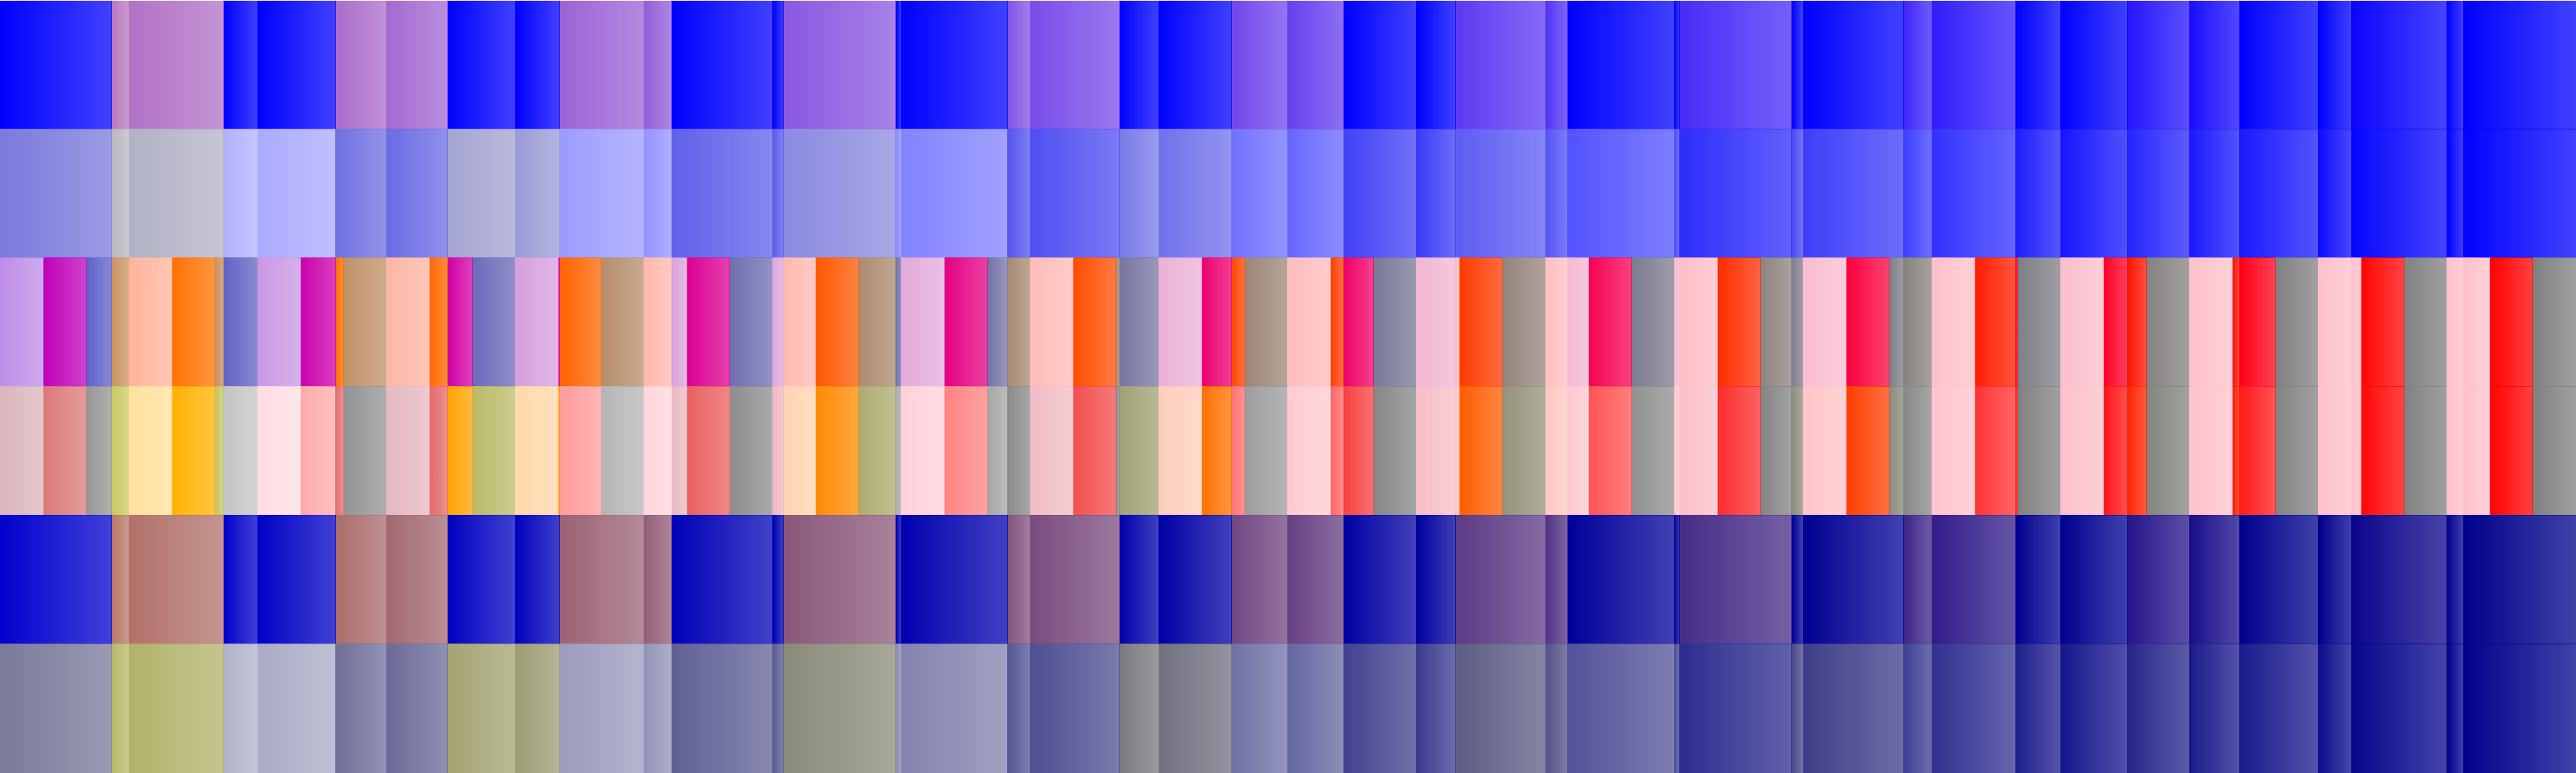
\includegraphics[width=0.45\textwidth]{figures/83bfba2f16ef59ec40127dd48d4c94e5_gradient_0.pdf}

Instead of using `fastcat', the above makes straightforward use of
Tidal's mini-notation for polyrhythmic sequences, denoted by double
quotes.

It is worth reiterating at this point that all these patterns are
functions, and not data structures. By combining them in this way we are
not computing anything, only creating a new function composed of other
functions, i.e.~composing behaviours. No calculation actually takes
place until the resulting pattern is queried.

\hypertarget{patterned-parameters}{%
\subsection{Patterned parameters}\label{patterned-parameters}}

TidalCycles has a large library of combinators, but for the purpose of
this paper we will focus on just one, the \texttt{fast} function, which
simply speeds up (or for factors \textless{} 1 slows down) a pattern.
Its definition is minimal, taking a time factor and a target pattern as
input, and manipulating the target pattern's timeline according to the
factor:

\begin{Shaded}
\begin{Highlighting}[]
\NormalTok{fast timepat pat }\OtherTok{=}
\NormalTok{  innerJoin ((\textbackslash{}time }\OtherTok{{-}>}\NormalTok{ withResultTime (}\OperatorTok{/}\NormalTok{ time) }\OperatorTok{$}
\NormalTok{                       withQueryTime (}\OperatorTok{*}\NormalTok{ time) pat)}
              \OperatorTok{<$>}\NormalTok{ timepat}
\NormalTok{            )}
\end{Highlighting}
\end{Shaded}

What is interesting in the above is that the time factor input is itself
a pattern. With combined use of the \texttt{\textless{}\$\textgreater{}}
operator and \texttt{innerJoin} function, we manipulate the target
pattern \emph{inside} the pattern of time. This higher order magic uses
much the same procedure to combine patterns as the one described
earlier. The result is a highly flexible function for patterning the
speed of a pattern. For example:

\begin{Shaded}
\begin{Highlighting}[]
\NormalTok{fast }\DecValTok{4} \OperatorTok{$}\NormalTok{ fast }\StringTok{"1 2 3"} \StringTok{"white pink red orange"}
\end{Highlighting}
\end{Shaded}


\includegraphics[width=0.45\textwidth]{figures/43220a67b5b9a766c3b9b0b23e6fec64_gradient_0.pdf}

The above switches between slices of the colour pattern running at
different speeds. An additional \texttt{fast} function is applied so
that you can see four cycles of the result. Once a few more simple
transformations are added, textures begin to form:

\begin{Shaded}
\begin{Highlighting}[]
\NormalTok{superimpose rev }\OperatorTok{$}\NormalTok{ superimpose (fast }\DecValTok{2}\NormalTok{)}
   \OperatorTok{$}\NormalTok{ chunk }\DecValTok{4}\NormalTok{ (blend }\FloatTok{0.5}\NormalTok{ red }\OperatorTok{<$>}\NormalTok{) }
   \OperatorTok{$}\NormalTok{ superimpose rev }
   \OperatorTok{$}\NormalTok{ fast }\StringTok{"1 5 3"} 
   \OperatorTok{$}\NormalTok{ iter }\DecValTok{4} \StringTok{"white pink red orange"}
\end{Highlighting}
\end{Shaded}

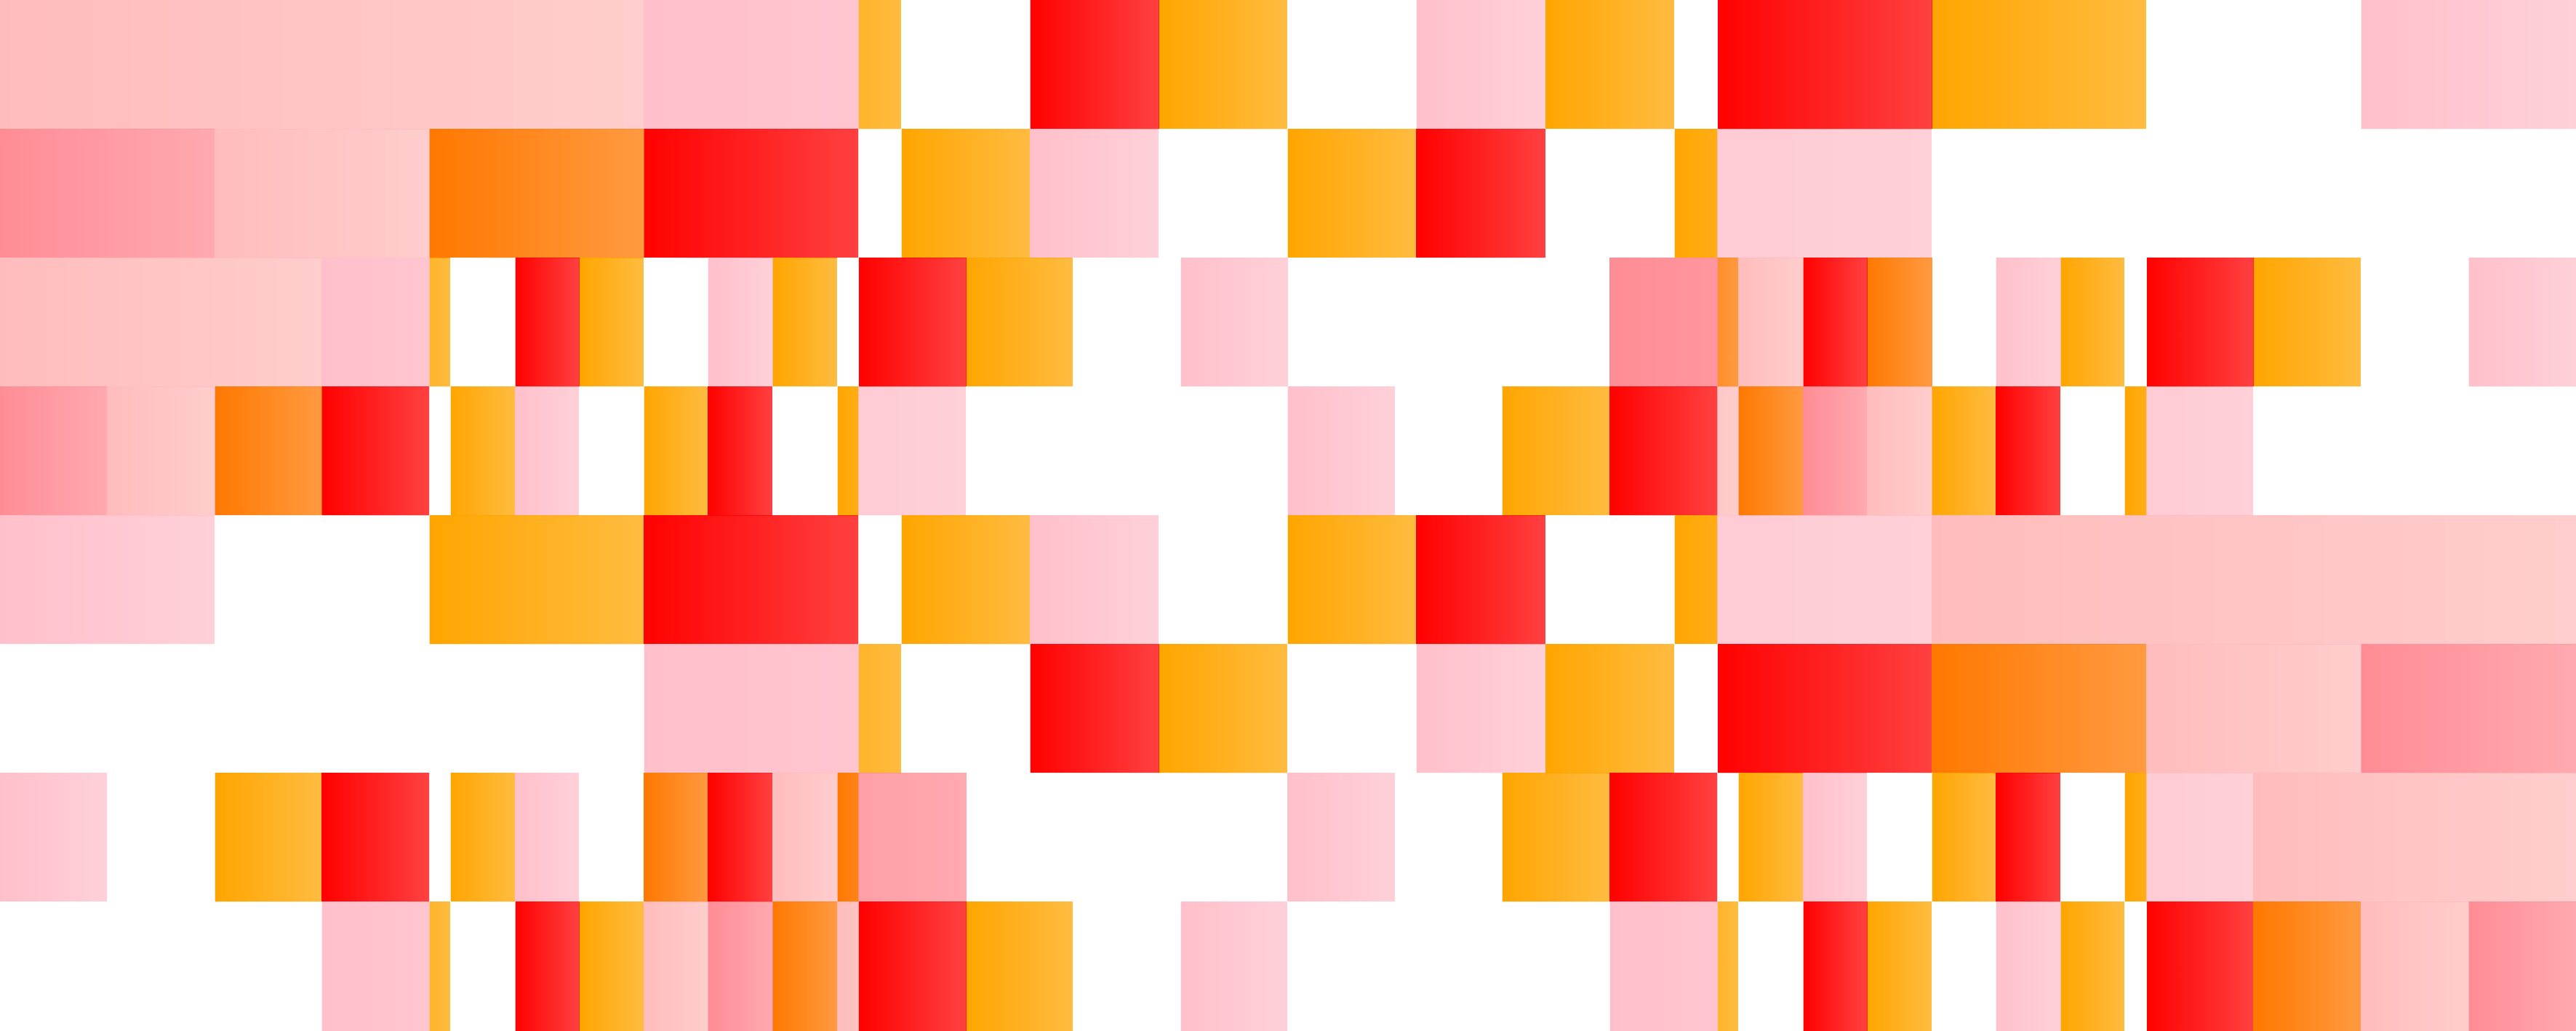
\includegraphics[width=0.45\textwidth]{figures/37d5734b7b2590f3dc2dcec00b8beaf5_gradient_0.pdf}

Again, the above code does not calculate anything on its own, it
composes together into a single function, which is then passed to the
scheduler (or in this case, graphics renderer) which queries the
required time arcs.

\hypertarget{tidalcycles-as-algorithmic-pattern-interface}{%
\subsection{TidalCycles as algorithmic pattern
interface}\label{tidalcycles-as-algorithmic-pattern-interface}}

Please refer to \href{https://tidalcycles.org}{tidalcycles.org} for
further details of Tidal's library of combinators, polyrhythmic
mini-notation, and independently patternable effects. But already, we
can see some of the affordances which Tidalcycles offers. Every part of
the above code example is trivial on its own, starting with a four-step
sequence, and adding simple transformations on top. However, the results
quickly become astonishingly complex, with each edit giving results
which become practically impossible to predict. This is because the
different elements interfere with each other, so that every simple part
has complex influence over the whole.

\hypertarget{algorithmic-pattern-in-hand-weaving}{%
\section{Algorithmic Pattern in Hand
Weaving}\label{algorithmic-pattern-in-hand-weaving}}

Hand weaving is an advanced world of technology, having developed over
thousands of years within diverse cultures of practice across the world.
All weaving is digital technology, in that it involves discrete crossing
points between warp (vertical) and weft (horizontal) threads. As with
Tidal, a weave involves interference between multiple interacting
systems. In other words, all weavers work with algorithmic patterns,
\emph{especially} hand weavers, who work without any machine or computer
to do calculations for them, so do it all themselves.

\hypertarget{colour-and-weave}{%
\subsection{Colour and weave}\label{colour-and-weave}}

It is difficult to get across the complexities of weave in a single
paper, but one clear example is the family of colour-and-weave effects,
where systems of colour and binary structure interfere to create the end
result (McLean and Harlizius-Klueck 2018). The following shows an
elementary example with a diagonal `twill' structure. The left shows the
weave `block' structure, a binary grid representing meeting points
between warp and weft threads. A square is black where a weft goes over
the warp, and white where it goes under. The central diagram shows a
simulation of this pattern woven with light weft and dark warp threads,
with the diagonal structure visible in the results. However, if we weave
the same structure with alternating light and dark threads on both the
warp and weft, the result (shown on the right) has the appearance of a
diagonal moving in a different direction. This is a trivial example of a
colour-and-weave effect, which can be exploited to create a wide range
of imagery from the same grid structure.

\begin{figure}[h]
\includegraphics[width=0.45\textwidth]{twill.png}
\end{figure}

\hypertarget{double-weave}{%
\subsection{Double weave}\label{double-weave}}

Working with weaves as a two dimensional binary structure is a useful
abstraction, but like all abstractions is not a complete model. The
threads of weaves move in three dimensions, with the structure of the
threads themselves, and their behaviour under tension, having strong
bearing on the end result. It is therefore a mistake to think that the
binary grid fully represents reality. Such a mistake seems to have been
made by Grünbaum and Shephard (1980), who approach weaving from the
point of view of two-dimensional tiling patterns. Using geometric rules,
they prove that the following weave structure result in a textile which
`falls apart':

\begin{figure}[h]
\includegraphics[width=0.45\textwidth]{grafik1.png}
\end{figure}

When this structure is `woven' using rigid card, this does appear to be
the case; half of the weave lifts off the rest, resulting in highly
unstable structures:

\includegraphics[width=0.45\textwidth]{card.png}

However as can be seen below, if we weave the structure with warp
threads under tension on a loom, we find that the two layers hold
together perfectly. Rather than `falling apart', the textile simply
splits in two. In fact, this technique of weaving two (or more) layers
at once is very well known by weavers as double (or triple, etc) weave,
resulting in a thick structure, where threads from the two layers can
exchange to create a range of effects.{[}\^{} The weave was itself live
coded, on the `live loom' (McLean 2020){]}

\begin{figure}[h]
\includegraphics[width=0.45\textwidth]{weave.jpg}
\end{figure}

\hypertarget{algorithmic-pattern-as-interface}{%
\section{Algorithmic Pattern as
Interface}\label{algorithmic-pattern-as-interface}}

To conclude, let's consider the place of algorithmic pattern as an
interface between a musician and their music. We have seen how the
algorithmic patterning of interference patterns within a two-dimensional
grid acts as an interface between weaver and weave. It allows
manipulation of textile at one-step removed, in terms of higher order
structure that can generate surprising results, including through
colour-and-weave and double weave effects. But when weaving we must
recognise that the block design is only one part of the whole, and that
to weave is both a computational and embodied experience where abstract
algorithmic patterns meet real-world behaviours. It is not possible to
understand a woven structure without actually weaving it.

The same lesson applies to algorithmic patterns in live coding. We can
work with the pattern as code, but it does not notate what we hear and
feel. Not only do interference patterns work inside the computer at
scales beyond our imaginations, but they then leave the computer as
sound, perceived as music in ways which do not exist in the notation but
in our embodied minds. Live coding involves an improvised movement of
pattern across cognition, computation and perception, a fundamentally
experimental activity, where code is developed in the open-minded and
open-bodied spirit of discovery. Without understanding that the
algorithm is only one step in the creation of music, we might find that
our music simply falls apart.

\hypertarget{acknowledgments}{%
\section{Acknowledgments}\label{acknowledgments}}

This research is conducted by the PENELOPE project, with funding from
the European Research Council (ERC) under the Horizon 2020 research and
innovation programme of the European Union, grant agreement No 682711.

\hypertarget{bibliography}{%
\section{Bibliography}\label{bibliography}}

\small

\hypertarget{refs}{}
\begin{cslreferences}
\leavevmode\hypertarget{ref-Rauber-Du-Bois2019}{}%
Bois, Andre Rauber Du, and Rodrigo Geraldo Ribeiro. 2019. ``HMusic: A
Domain Specific Language for Music Programming and Live Coding.'' In
\emph{Proceedings of the International Conference on New Interfaces for
Musical Expression}, edited by Marcelo Queiroz and Anna Xambó Sedó,
381--86. Porto Alegre, Brazil: UFRGS.
\url{http://www.nime.org/proceedings/2019/nime2019_paper074.pdf}.

\leavevmode\hypertarget{ref-Bouillot2007}{}%
Bouillot, Nicolas. 2007. ``NJam User Experiments : Enabling Remote
Musical Interaction from Milliseconds to Seconds.'' In \emph{Proceedings
of the International Conference on New Interfaces for Musical
Expression}, 142--47. New York City, NY, United States.
\url{http://www.nime.org/proceedings/2007/nime2007_142.pdf}.

\leavevmode\hypertarget{ref-ncollins2014}{}%
Collins, Nick, and Alex McLean. 2014. ``Algorave: Live Performance of
Algorithmic Electronic Dance Music.'' In \emph{Proceedings of the
International Conference on New Interfaces for Musical Expression},
355--58. London, United Kingdom: Goldsmiths, University of London.
\url{http://www.nime.org/proceedings/2014/nime2014_426.pdf}.

\leavevmode\hypertarget{ref-Derbinsky2012}{}%
Derbinsky, Nate, and Georg Essl. 2012. ``Exploring Reinforcement
Learning for Mobile Percussive Collaboration.'' In \emph{Proceedings of
the International Conference on New Interfaces for Musical Expression}.
Ann Arbor, Michigan: University of Michigan.
\url{http://www.nime.org/proceedings/2012/nime2012_241.pdf}.

\leavevmode\hypertarget{ref-Eigenfeldt2008}{}%
Eigenfeldt, Arne, and Ajay Kapur. 2008. ``An Agent-Based System for
Robotic Musical Performance.'' In \emph{Proceedings of the International
Conference on New Interfaces for Musical Expression}, 144--49. Genoa,
Italy. \url{http://www.nime.org/proceedings/2008/nime2008_144.pdf}.

\leavevmode\hypertarget{ref-Elliott09}{}%
Elliott, Conal. 2009. ``Push-Pull Functional Reactive Programming.'' In
\emph{Proceedings of 2nd Acm Sigplan Symposium on Haskell 2009}.

\leavevmode\hypertarget{ref-cfaubel12014}{}%
Faubel, Christian. 2014. ``Rhythm Apparatus on Overhead.'' In
\emph{Proceedings of the International Conference on New Interfaces for
Musical Expression}, 491--94. London, United Kingdom: Goldsmiths,
University of London.
\url{http://www.nime.org/proceedings/2014/nime2014_503.pdf}.

\leavevmode\hypertarget{ref-Fell18}{}%
Fell, Mark. 2018. ``Notes on Pattern Synthesis: 1983 to 2013.'' In,
edited by Alex McLean and Roger Dean. Oxford University Press.

\leavevmode\hypertarget{ref-Gimenes2007}{}%
Gimenes, Marcelo, Eduardo Miranda, and Chris Johnson. 2007.
``Musicianship for Robots with Style.'' In \emph{Proceedings of the
International Conference on New Interfaces for Musical Expression},
197--202. New York City, NY, United States.
\url{http://www.nime.org/proceedings/2007/nime2007_197.pdf}.

\leavevmode\hypertarget{ref-ogreen2014}{}%
Green, Owen. 2014. ``NIME, Musicality and Practice-Led Methods.'' In
\emph{Proceedings of the International Conference on New Interfaces for
Musical Expression}, 1--6. London, United Kingdom: Goldsmiths,
University of London.
\url{http://www.nime.org/proceedings/2014/nime2014_434.pdf}.

\leavevmode\hypertarget{ref-Greunbaum86}{}%
Grünbaum, Branko, and G C Shephard. 1986. \emph{Tilings and Patterns}.
USA: W. H. Freeman \& Co.

\leavevmode\hypertarget{ref-Gruenbaum80}{}%
Grünbaum, Branko, and Geoffrey C. Shephard. 1980. ``Satins and Twills:
An Introduction to the Geometry of Fabrics.'' \emph{Mathematics
Magazine} 53 (3): 139--61. \url{http://www.jstor.org/stable/2690105}.

\leavevmode\hypertarget{ref-Hawryshkewich2010}{}%
Hawryshkewich, Andrew, Philippe Pasquier, and Arne Eigenfeldt. 2010.
``Beatback : A Real-Time Interactive Percussion System for Rhythmic
Practise and Exploration.'' In \emph{Proceedings of the International
Conference on New Interfaces for Musical Expression}, 100--105. Sydney,
Australia. \url{http://www.nime.org/proceedings/2010/nime2010_100.pdf}.

\leavevmode\hypertarget{ref-Jordnicode2252016}{}%
Jordà, Sergi, Daniel Gómez-Marín, Ángel Faraldo, and Perfecto Herrera.
2016. ``Drumming with Style: From User Needs to a Working Prototype.''
In \emph{Proceedings of the International Conference on New Interfaces
for Musical Expression}, 16:365--70. 2220-4806. Brisbane, Australia:
Queensland Conservatorium Griffith University.
\url{http://www.nime.org/proceedings/2016/nime2016_paper0071.pdf}.

\leavevmode\hypertarget{ref-Kim2013}{}%
Kim, Taehun, and Stefan Weinzierl. 2013. ``Modelling Gestures in Music
Performance with Statistical Latent-State Models.'' In \emph{Proceedings
of the International Conference on New Interfaces for Musical
Expression}, 427--30. Daejeon, Republic of Korea: Graduate School of
Culture Technology, KAIST.
\url{http://nime.org/proceedings/2013/nime2013_244.pdf}.

\leavevmode\hypertarget{ref-Kitani2010}{}%
Kitani, Kris M., and Hideki Koike. 2010. ``ImprovGenerator : Online
Grammatical Induction for on-the-Fly Improvisation Accompaniment.'' In
\emph{Proceedings of the International Conference on New Interfaces for
Musical Expression}, 469--72. Sydney, Australia.
\url{http://www.nime.org/proceedings/2010/nime2010_469.pdf}.

\leavevmode\hypertarget{ref-Lee2007}{}%
Lee, Eric, Urs Enke, Jan Borchers, and Leo de Jong. 2007. ``Towards
Rhythmic Analysis of Human Motion Using Acceleration-Onset Times.'' In
\emph{Proceedings of the International Conference on New Interfaces for
Musical Expression}, 136--41. New York City, NY, United States.
\url{http://www.nime.org/proceedings/2007/nime2007_136.pdf}.

\leavevmode\hypertarget{ref-Lee2006}{}%
Lee, Eric, Ingo Grüll, Henning Keil, and Jan Borchers. 2006. ``Conga: A
Framework for Adaptive Conducting Gesture Analysis.'' In
\emph{Proceedings of the International Conference on New Interfaces for
Musical Expression}, 260--65. Paris, France.
\url{http://www.nime.org/proceedings/2006/nime2006_260.pdf}.

\leavevmode\hypertarget{ref-Lee:2012a}{}%
Lee, Sang Won, Jason Freeman, and Andrew Collela. 2012. ``Real-Time
Music Notation, Collaborative Improvisation, and Laptop Ensembles.'' In
\emph{Proceedings of the International Conference on New Interfaces for
Musical Expression}. Ann Arbor, Michigan: University of Michigan.
\url{http://www.nime.org/proceedings/2012/nime2012_62.pdf}.

\leavevmode\hypertarget{ref-slui2014}{}%
Lui, Simon. 2014. ``A Real Time Common Chord Progression Guide on the
Smartphone for Jamming Pop Song on the Music Keyboard.'' In
\emph{Proceedings of the International Conference on New Interfaces for
Musical Expression}, 98--101. London, United Kingdom: Goldsmiths,
University of London.
\url{http://www.nime.org/proceedings/2014/nime2014_275.pdf}.

\leavevmode\hypertarget{ref-mclean_live_2020}{}%
McLean, Alex. 2020. ``The Live Loom.'' In \emph{Proceedings of the 5th
International Conference on Live Coding}. Limerick, Ireland: University
of Limerick.

\leavevmode\hypertarget{ref-McLean18}{}%
McLean, Alex, and Ellen Harlizius-Klueck. 2018. ``Digital Art: A Long
History.'' In \emph{Proceedings of the International Conference on Live
Interfaces}, 71--77.

\leavevmode\hypertarget{ref-McLean18b}{}%
McLean, Alex, and Ellen Harlizius-Klück. 2018. ``Fabricating Algorithmic
Art.'' Austrian Cultural Forum.
\url{https://doi.org/10.5281/zenodo.2155745}.

\leavevmode\hypertarget{ref-Ogawa2009}{}%
Ogawa, Keisuke, and Yasuo Kuhara. 2009. ``Life Game Orchestra as an
Interactive Music Composition System Translating Cellular Patterns of
Automata into Musical Scales.'' In \emph{Proceedings of the
International Conference on New Interfaces for Musical Expression},
50--51. Pittsburgh, PA, United States.
\url{http://www.nime.org/proceedings/2009/nime2009_050.pdf}.

\leavevmode\hypertarget{ref-Petit2019}{}%
Petit, Bertrand, and manuel serrano. 2019. ``Composing and Executing
Interactive Music Using the Hiphop.js Language.'' In \emph{Proceedings
of the International Conference on New Interfaces for Musical
Expression}, edited by Marcelo Queiroz and Anna Xambó Sedó, 71--76.
Porto Alegre, Brazil: UFRGS.
\url{http://www.nime.org/proceedings/2019/nime2019_paper014.pdf}.

\leavevmode\hypertarget{ref-Schoonderwaldt2011}{}%
Schoonderwaldt, Erwin, and Alexander Refsum Jensenius. 2011. ``Effective
and Expressive Movements in a French-Canadian Fiddler's Performance.''
In \emph{Proceedings of the International Conference on New Interfaces
for Musical Expression}, 256--59. Oslo, Norway.
\url{http://www.nime.org/proceedings/2011/nime2011_256.pdf}.

\leavevmode\hypertarget{ref-Sicchio14}{}%
Sicchio, Kate. 2014. ``Data Management Part III: An Artistic Framework
for Understanding Technology Without Technology.'' Edited by Pat Badani,
Kevin Hamilton, and Terri Weissman. \emph{Media-N: Journal of the New
Media Caucus} 10 (3).

\leavevmode\hypertarget{ref-Spiegel81}{}%
Spiegel, Laurie. 1981. ``Manipulations of Musical Patterns.'' In
\emph{Proceedings of the Symposium on Small Computers and the Arts},
19--22.

\leavevmode\hypertarget{ref-Subramanian2012}{}%
Subramanian, Sidharth, Jason Freeman, and Scott McCoid. 2012. ``LOLbot:
Machine Musicianship in Laptop Ensembles.'' In \emph{Proceedings of the
International Conference on New Interfaces for Musical Expression}. Ann
Arbor, Michigan: University of Michigan.
\url{http://www.nime.org/proceedings/2012/nime2012_119.pdf}.

\leavevmode\hypertarget{ref-Suiter2010}{}%
Suiter, Wendy. 2010. ``Toward Algorithmic Composition of Expression in
Music Using Fuzzy Logic.'' In \emph{Proceedings of the International
Conference on New Interfaces for Musical Expression}, 319--22. Sydney,
Australia. \url{http://www.nime.org/proceedings/2010/nime2010_319.pdf}.

\leavevmode\hypertarget{ref-Toka2018}{}%
Toka, Mert, Can Ince, and Mehmet Aydin Baytas. 2018. ``Siren: Interface
for Pattern Languages.'' In \emph{Proceedings of the International
Conference on New Interfaces for Musical Expression}, edited by Thomas
Martin Luke Dahl Douglas Bowman, 53--58. Blacksburg, Virginia, USA:
Virginia Tech.
\url{http://www.nime.org/proceedings/2018/nime2018_paper0014.pdf}.

\leavevmode\hypertarget{ref-Trail:2012a}{}%
Trail, Shawn, Michael Dean, Gabrielle Odowichuk, Tiago Fernandes
Tavares, Peter Driessen, W. Andrew Schloss, and George Tzanetakis. 2012.
``Non-Invasive Sensing and Gesture Control for Pitched Percussion
Hyper-Instruments Using the Kinect.'' In \emph{Proceedings of the
International Conference on New Interfaces for Musical Expression}. Ann
Arbor, Michigan: University of Michigan.
\url{http://www.nime.org/proceedings/2012/nime2012_297.pdf}.

\leavevmode\hypertarget{ref-rvogl2017}{}%
Vogl, Richard, and Peter Knees. 2017. ``An Intelligent Drum Machine for
Electronic Dance Music Production and Performance.'' In
\emph{Proceedings of the International Conference on New Interfaces for
Musical Expression}, 251--56. Copenhagen, Denmark: Aalborg University
Copenhagen.
\url{http://www.nime.org/proceedings/2017/nime2017_paper0047.pdf}.
\end{cslreferences}



\end{document}
